\documentclass{article}
\usepackage{adjustbox}
\usepackage{float}
\usepackage{wrapfig}
\usepackage{polski}
\usepackage[utf8]{inputenc}
\usepackage{polski}
\usepackage{amssymb}
\usepackage{color}
\usepackage{amsmath}
\usepackage{enumerate}
\usepackage{hyperref}
\usepackage{listings}
\lstset{language=R}


\title{Analiza najdroższych transferów piłkarskich}
\author{\textbf{Paweł Gorgolewski}\\ 
\textit{AGH, Wydział Informatyki Elektroniki i Telekomunikacji}\\
\textit{Rachunek prawdopodobieństwa i statystyka 2021/2022}}
\date{Kraków, \today}


\begin{document}
\maketitle

\textit{Ja, niżej podpisany własnoręcznym podpisem deklaruję, że przygotowałem(łam) przedstawiony do oceny projekt samodzielnie i żadna jego część nie jest kopią pracy innej osoby.}
\begin{flushright}
{............................................}
\end{flushright}

\section{Streszczenie raportu}
Raport powstał w oparciu o bazę danych: \href{url}{https://www.kaggle.com/berkayalan/the-most-expensive-football-transfers} i ma na celu przeanalizowanie 54 najdroższych transferów w piłce nożnej

\section{Opis danych}
Dane zawierają 54 najdroższych piłkarzy w historii. Kazdy rekord ma następujące cechy:
\begin{itemize}
    \item \textbf{Rank} - numer w rankingu
    \item \textbf{Origin} - kraj pochodzenia piłkarza
    \item \textbf{Player} - imię i nazwisko piłkarza
    \item \textbf{From.Country.} - kraj z której ligi odchodził piłkarz
    \item \textbf{From.Club.} - klub z której ligi odchodził piłkarz
    \item \textbf{To.Country.} - kraj do której ligi przeniósł się piłkarz
    \item \textbf{To.Club.} - klub do którego przeniósł się piłkarz
    \item \textbf{Position} - pozycja na której gra piłkarz
    \item \textbf{Fee...mln.} - cena trasferu w Euro
    \item \textbf{Fee.L.mln.} - cena transferu w Funtach
    \item \textbf{Year} - rok transferu
    \item \textbf{Born} - rok urodzenia piłkarza
\end{itemize}

Część z tych danych nie podobała mi się (nazwy także) więc zdecydowałem się zdefiniować swoje własne dane na podstawie wyżej wymienionych. Każdy rekord z przedefiniowanych danych to:
\begin{itemize}
    \item \textbf{Player} - imię i nazwisko piłkarza
    \item \textbf{Origin} - kraj pochodzenia piłkarza
    \item \textbf{From\textunderscore Country} - kraj z której ligi odchodził piłkarz
    \item \textbf{From\textunderscore Club} - klub z której ligi odchodził piłkarz
    \item \textbf{To\textunderscore Country} - kraj do której ligi przeniósł się piłkarz
    \item \textbf{To\textunderscore Club} - klub do którego przeniósł się piłkarz
    \item \textbf{Position} - pozycja na której gra piłkarz
    \item \textbf{Fee\textunderscore Euro} - cena trasferu w milionach Euro
    \item \textbf{Age} - wiek piłkarza w momencie transferu (czyli 'Year'-'Born')
\end{itemize}

\section{Analiza danych}
\subsection{Wstępne rozeznanie się w danych}
Na sam początek, warto sprawdzić jak wyglądają podstawowe statystki związane z naszymi danymi numerycznymi, czyli \textit{Age} oraz \textit{Fee\textunderscore Euro}

Poniżej statystyki dla \textit{Age}

\begin{figure}[H]
    \centering
    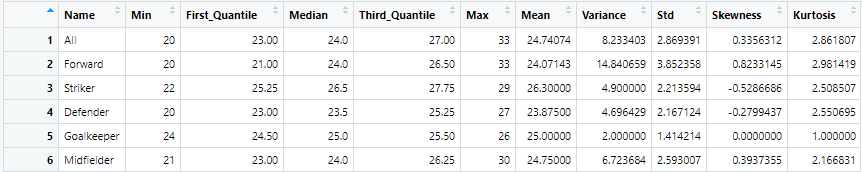
\includegraphics[width=1\linewidth]{age_stats.png}
\end{figure}

Widząc statystki dla cechy \textit{Age} można zauważyć:
\begin{enumerate}
    \item Najbardziej rozproszoną wiekowo grupą wokół średniej są zawodnicy ofensywni
    \item Najmniej rozporoszoną wiekowo grupą wokół średniej są bramkarze (tak na marginesie jest ich tylko 2)
    \item Rozkład (ze skośności):
    \begin{itemize}
        \item jest symetryczny dla bramkarzy
        \item ma długi ogon prawostronny dla napastników pomocników i zestawieniu wszystkich zawodników
        \item ma długi ogon lewostronny dla obrońców i napastników
    \end{itemize}
    \item Rozkład (z kurtozy): dla każdego przypadków w danych istnieje więcej dodatnich wartości odstających niż w przypadku rozkładu normalnego
\end{enumerate}

Teraz spójrzmy na statystyki czegoś bardziej interesującego - pieniędzy, czyli \textit{Fee\textunderscore Euro}:

\begin{figure}[H]
    \centering
    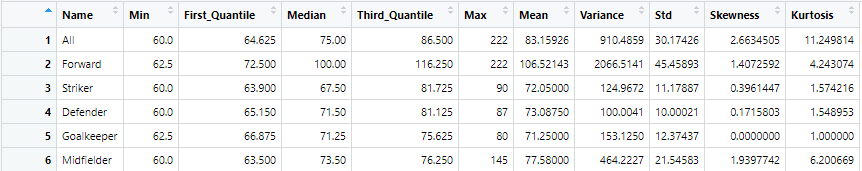
\includegraphics[width=1\linewidth]{fee_stats.png}
\end{figure}

Rozważając te same statystyki dla \textit{Fee\textunderscore Euro}:
\begin{enumerate}
    \item Najbardziej rozproszoną grupą pod względem kosztu transferu wokół średniej są zawodnicy ofensywni
    \item Najmniej rozporoszoną grupą pod względem kosztu trasferu wokół średniej są obrońcy
    \item Rozkład (ze skośności):
    \begin{itemize}
        \item jest symetryczny dla bramkarzy
        \item ma długi ogon prawostronny dla reszty grup (zauważmy, że obrońcy mają prawie symetryczny rozkład - skośność bliska 0)
    \end{itemize}
    \item Rozkład (z kurtozy): dla każdego przypadków w danych istnieje więcej dodatnich wartości odstających niż w przypadku rozkładu normalnego
\end{enumerate}

Łatwo zauważyć, że maksymalna kwota transferu to aż 222 miliony Euro! Patrząc na takie sumy aż chce się zobaczyć TOP 10 najdroższych transferów w piłce nożnej. Oto one:

\begin{figure}[H]
    \centering
    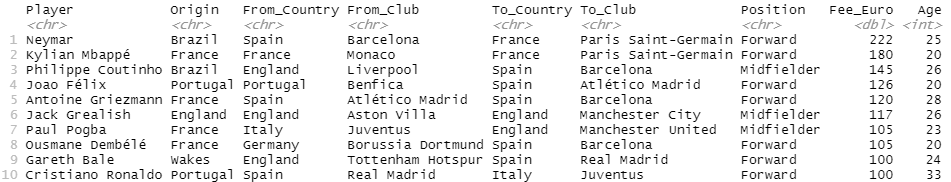
\includegraphics[width=1\linewidth]{Top10_players.png}
\end{figure}

Porównując teraz wcześniejsze statystki i TOP 10 transferów dzieje się coś zadziwiającego. Jak to się stało, że drugi najdroższy piłkarz świata to najmłodszy w zestawieniu 20-latek!? Tak samo może ktoś spytać, dlaczego na 10 miejscu znajduje się najstarszy piłkarz (33 lat) i to za aż 100 milionów Euro!
Dodatkowo, jeśli kogoś nie interesuje tylko wiek piłkarza i kwota transferu - prawie wszyscy zawodnicy w TOP 10 są piłkarzami ofensywnymi. 

W tym tkwi sedno problemu, w najdroższych transferach często nie chodzi tylko o umiejętności piłkarza i wiek, ale także jego rozpoznawalność, klub do jakiego oraz z jakiego przychodzi a także pozycja na której występuje. To czego nie ma w bazie, ale też ma znaczenie to długośc obecnego kontraktu (im krótszy kontrakt ma piłkarz tym mniej się za niego płaci - po skończeniu kontraktu można go wziąc za darmo. Przykład Lewandowski z Borussi do Bayernu)

\subsection{Pozycja zawodnika a cena}
Wiemy, że Neymar i Mbappe to najdrożsi piłkarze na świecie oraz oboje są są zawodnikami ofensywnymi. Z poprzednich statystyk wiemu już nieco o podziale na pozycję, lecz mimo wszystko zilustrujmy to sobie:

\begin{figure}[H]
    \centering
    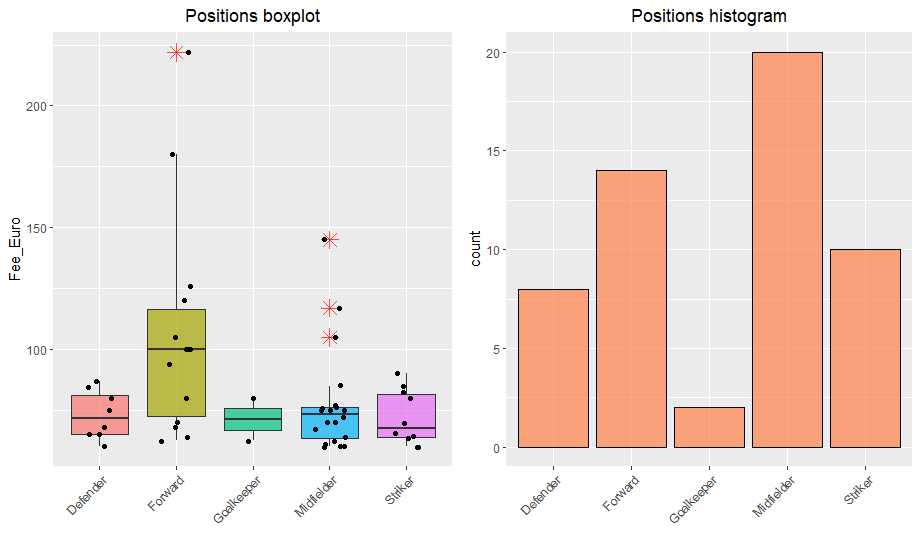
\includegraphics[width=1\linewidth]{postions_boxplot_histogram.png}
\end{figure}

Tak jak wcześniej można było wywnioskować ze statystyk - zdecydowanie najdrożsi są zawodnicy ofensywni. Reszta pozycji nie ma większej różnicy między sobą - można wyróżnić tylko bramkarzy, ponieważ istnieją tylko 2 transfery z tej pozycji co jest lekko niemiarodajne. Ku mojemu zdziwiemiu, kupiono więcej pomocników niż atakujących! Oczywiście tak jak widać istnieją wyjątki od reguły i widać to na boxplotach - są to ceny zawodników które nie pasują do pozostałych w swojej kategorii. Ceny trzech pomocników i jednego z zawodników ofensywnych zdefiniowano jako wartości odstające (czerwone gwiazdki)

\subsection{Kraj z jakiego przybywa zawodnik a cena}
Nasze wiadomości rozszerzyły się o różnice między pozycjami. Jak wygląda sytuacja, gdy w podobny sposób rozważymy kraj z którego przybywa zawodnik?

\begin{figure}[H]
    \centering
    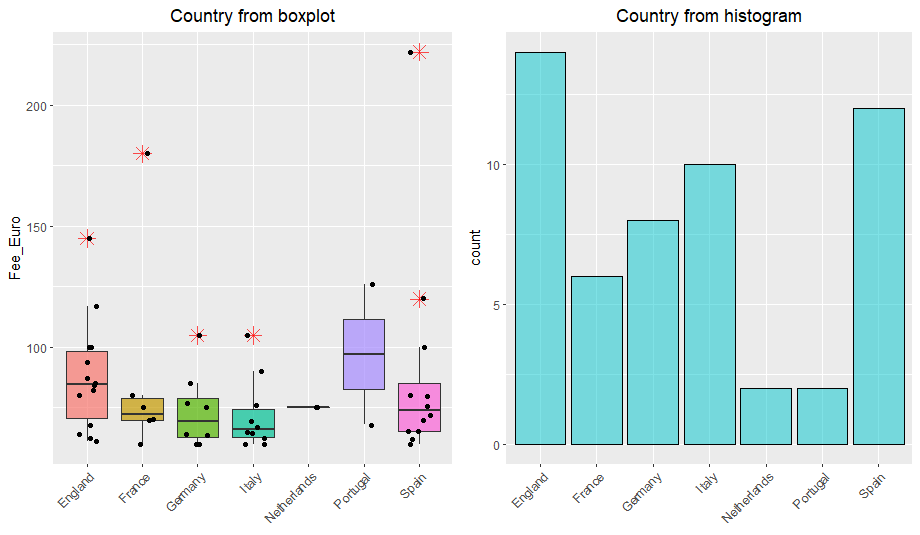
\includegraphics[width=1\linewidth]{country_from_boxplot_histogram.png}
\end{figure}

Tak jak widac na histogramie, niemalże wszystkie transfery są z TOP 5 lig europejskch: Anglia, Hiszpania, Niemcy, Włochy, Francja. Są też po dwa transfery z Portugalii oraz Holandii ale można z tego wysunąc prosty wniosek - tych 4 piłkarzy musiało się wybitnie wyróżniać na tle drużyny. A teraz dlaczego głównie z najmocniejsyzch lig? Odpowiedź jest prosta - piłkarz wyróżniający się w mocnej lidze, najprawdopodbniej bez problemu poradzi sobie w innej (bądź tej samej) mocnej lidze i będzie odgrywał w niej pierwszoplanową rolę.

Mimo jednego 'outliera' z Francji to Anglia i Hiszpania ma najbardziej cenionych piłkarzy na świecie, z przewagą angielską. Hiszpanią rządzi fakt posiadania dwóch klubów: Barcelony oraz Realu Madryt. Anglia ma 6 topowych i bogatych drużyn, zaś reszta ligii to również mocne zespoły. Nie bez powodu kursy u bukmacherów są wysokie na mecze tej ligi - tam każdy może wygrać z każdym (trochę jak nasza Ekstraklasa ale o wiele lepsze mecze)

\subsection{Kraj do którego przybywa zawodnik a cena}
Wiemy, że to piłkarze z Anglii i Hiszpanii są najbardziej cenieni. A gdzie najwięcej piłkarzy odchodzi ze swoich klubów?

\begin{figure}[H]
    \centering
    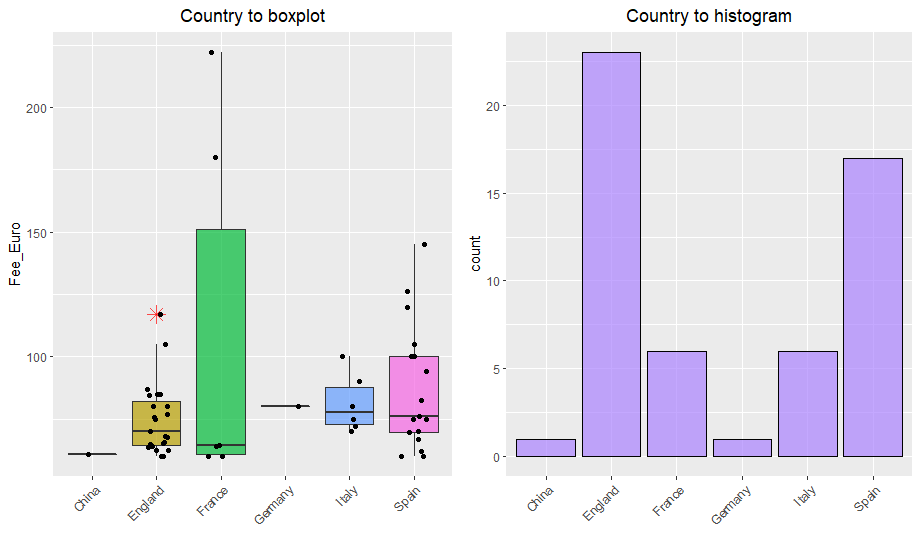
\includegraphics[width=1\linewidth]{country_to_boxplot_histogram.png}
\end{figure}

No i tym razem bez zaskoczenia - do Anglii. Pod względem liczebności transferów, tylko Hiszpania jako tako jej dorównuje. Jeżeli jednak popatrzymy na ceny transferów, to Hiszpania i Włochy są na najwyższym poziomie (mimo wszystko faworyzowałbym Hiszpanię przez o wiele większą liczbę transferów)

Patrząc na wykresy, można dostać lekkiego szoku. Dlaczego Neymar i Mbappe, czyli dwóch najdroższych zawodników na świecie, udali się do Francji? Oboje są świetnymi piłkarzami, więc dlaczego nie chcieli iśc do Anglii czy Hiszpanii? W praktyce chodziło tu o kwestie osobiste (Neymar chciał być numerem 1, Mbappe chciał zostać we Francji) oraz standardowo, o pieniądze - tylko klub PSG był w stanie zapłacić tak kosmiczne pieniądze za piłkarzy i dać im odpowiednie pensje.


\subsection{Kraje z których pochodzą zawodnicy a cena}
Neymar pochodzi z Brazylii, Mbappe z Francji. Wiemy już że ich ceny są mało porównywalne do reszty, lecz sprawdzić zawsze warto - jakiego pochodzenia piłkarzy kupuje się najdrożej.

\begin{figure}[H]
    \centering
    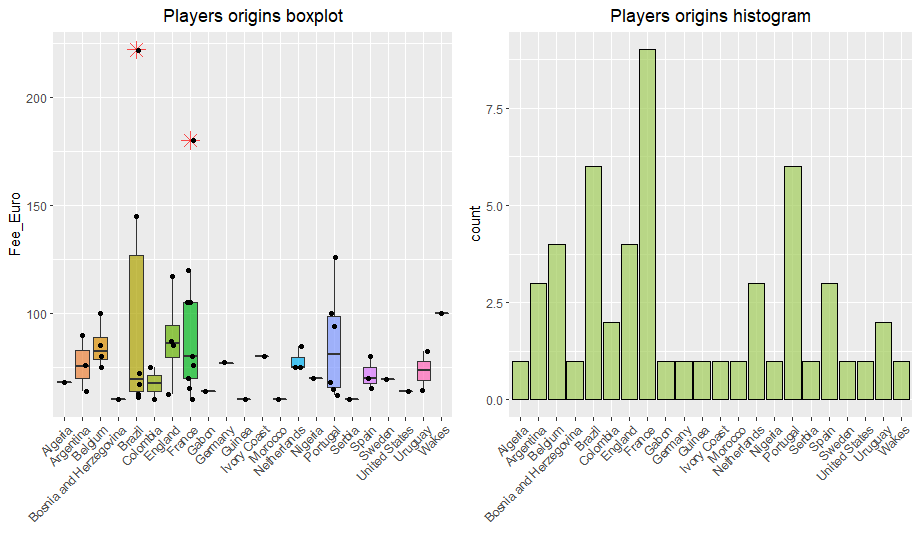
\includegraphics[width=1\linewidth]{origins_boxplot_histogram.png}
\end{figure}

Wyróżniającym się krajem jest Francja - ma najwięcej transferów. Brazylia i Portugalia dopełniają podium. Oprócz tego, żaden z krajów nie wyróznia się niczym szczególnym (poza Brazylią i Francją które mają swoje rekordowe transfery). Można zatem stwierdzić, że kraj pochodzenia nie ma większego znaczenia jeżeli chodzi o cenę transferu (równie dobrze zamiast Neymara za 222 mln mógły się tam znaleźć super wybitny gracz z Polski czy San Marino). Jedyne co tutaj gra rolę to prawdopodobieństwo wystąpienia tak drogiego (czyli uzdolnionego) zawodnika dla danej narodowości - tak jak każdy się spodziewa dla San Marino na pewno będzie jednym z najmniejszych.

\subsection{Kluby - przychód i wydatki z wielkich transferów}
A co gdyby ktoś się zastanawiał - jak wypadł każdy z klubów pod względem finansowym w tym zestawieniu?
Wiedząc, że PSG kupiło Mbappe i Neymara, zakładam, że ten klub będzie miał większy wydatki niż przychody. Zobaczmy jak to się ma dla każdego z klubów:

\begin{figure}[H]
    \centering
    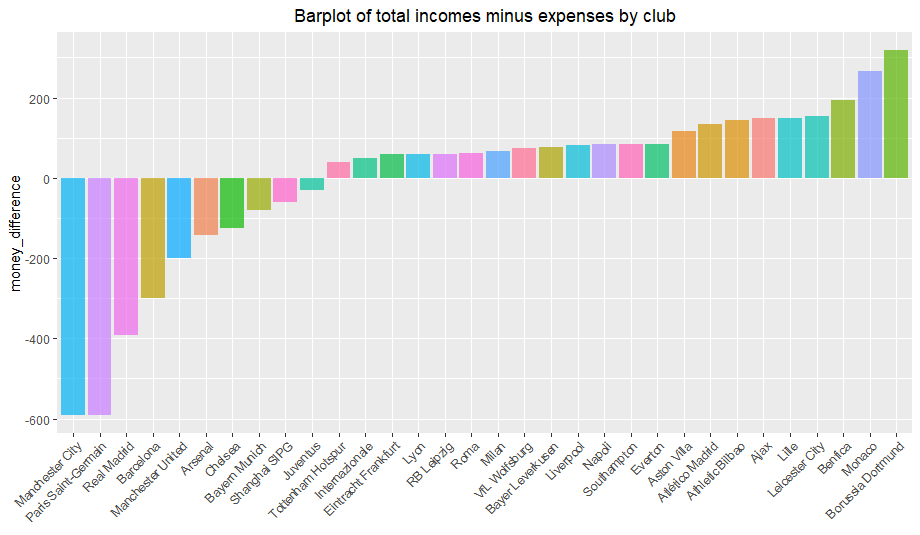
\includegraphics[width=1\linewidth]{incomes_minus_expenses.png}
\end{figure}

Tak jak to było wcześniej powiedziane, drogie transfery wykonywane są tylko do mocnych lig i/lub bogatych zespołów. Nikogo tu pewnie nie dziwi, że 'na minusie' są takie kluby jak: Manchester City, PSG, Chelsea, Real Madryt, Barcelona. Z drugiej strony na plusie są zespoły które są mocne, grają w dobrych/najlepszych ligach ale nie są w stanie walczyć o ligę mistrzów, zapłacić wymaganej przez piłkarza pensji lub tak jak Ajax są nastawione na szkolenie wybitnych młodych piłkarzy i później ich sprzedawać (np. Ibrahimović). 

\subsection{Korelacja zmiennych}
Będąc przy transferach, nie można zapomnieć o rozważeniu czy wiek i cena idą ze sobą w parze. Poniżej przedstawiam macierze korelacji dla wieku i kwoty transferu:

\begin{figure}[H]
    \centering
    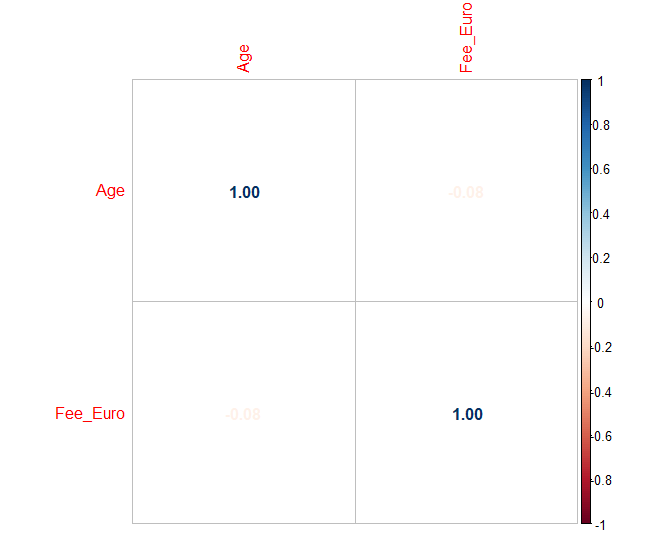
\includegraphics[width=1\linewidth]{linear_correlation.png}
\end{figure}

No i tak jak można się było spodziewać - może i jest jakieś powiązanie między tymi zmiennymi, ale na pewno nie jest ono liniowe.

\subsection{Gęstości i testy przynależności do rozkładu}
Rozważmy teraz gęstości naszych rozkładów z podziałem na pozycje:

\begin{figure}[H]
    \centering
    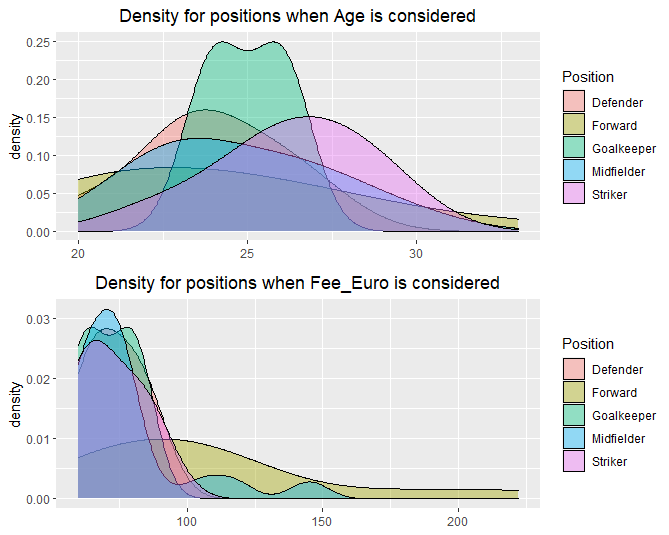
\includegraphics[width=.8\linewidth]{densities.png}
\end{figure}

Nie można ukryć, wyglądają ciekawie. Tak samo interesujące jest, czy po połączeniu (czyli wyliczeniu gęstości dla wszystkich zawodników w bazie) dostaniemy rozkłady podobne do normalnego. Spójrzmy na kolejne dwa wykresy:
\begin{figure}[H]
    \centering
    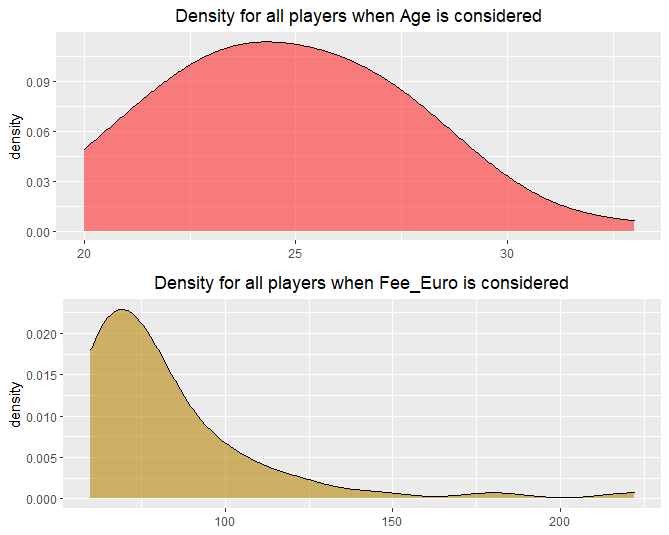
\includegraphics[width=.8\linewidth]{density_for_all_players.png}
\end{figure}

Zacznijmy od rozkładu przy rozważanym wieku piłkarza. Aby sprawdzić, czy rozkład jest normalny użyję testu \textit{Shapiro-Wilk'a}. Jeżeli wartość p będzie większa niż 0.05 (wartość tą zmienia się dla wartości $W>0.98$) to rozkład można uznawać za normalny.
\begin{figure}[H]
    \centering
    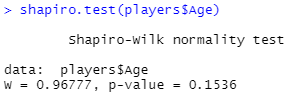
\includegraphics[width=.5\linewidth]{shapiro_test_for_ages.png}
\end{figure}
Wyniku testu są pozytywne - rozkład wieku piłkarzy można traktować jako rozkład normalny.

Teraz czas na sprawdzenie rozkładu ceny piłkarzy. Wszystko zadziała tutaj w analogiczny sposób, lecz spodziewamy się wartości $p<0.05$ - wykres gęstości o wiele mniej przypomina rozkład normalny. Spójrzmy na wyniki:
\begin{figure}[H]
    \centering
    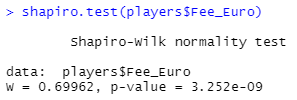
\includegraphics[width=.5\linewidth]{shapiro_test_for_fee.png}
\end{figure}
Wyniki testów potwierdzają przypuszczenia. P jest zdecydowanie mniejsze od 0.05 więc rozkład ten nie może być rozkładem normalnym.


\section{Wnioski}
Wnioski płynące z przeprowadzonej analizy, są następujące:
\begin{itemize}
\item Najbardziej pożądani są gracze ofensywni
\item Francja ma najliczniejszą reprezentację w zestawieniu najdroższych zawodników
\item Bogate i czołowe kluby wydają najwięcej na rekordowych transferach
\item Kluby z dobrą szkółką młodzieżową (np. Ajax) oraz kluby o dużym potencjale (np. Borussia) mają największy porfit z rekordowych transferów
\item Tak drodzy piłkarze zazwyczaj nie skończyli 30 lat
\item Zależnośc między wiekiem a ceną na pewno nie jest liniowa
\item Rozkład wieku piłkarzy można traktować jako rozkład normalny
\end{itemize}

\end{document}
